%2章
\chapter{提案手法}

本研究で対象とするエージェントシミュレーションの大きな特徴は,介護の対象となる高齢者の運動機能や認知機能の低下に大きなバリエーションがあると同時にも,介護者側にも国家資格をもった介護福祉士から,介護ヘルパー,ボランチィアスタッフまで技能や知識,経験に大きなバリエーションがあることである.そうしたことを念頭に置いた上で,本研究では介護者エージェント,被介護エージェント,環境としての高齢者施設の基本モデリングを検討した.図\ref{concept_simulation}に概念図を示す.黒で示される介護者が、自身が持つ視野の中で水色で示される被介護者を観測する.

\begin{figure}[htb]
\begin{center}
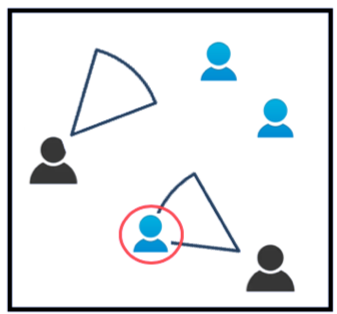
\includegraphics[scale=2.0]{figures/concept_simulation.png}
\caption[シミュレーションの概念図]{シミュレーションの概念図 \label{concept_simulation}}
\end{center}
\end{figure}

\section{知的マルチエージェントモデル}

介護行動は社会系の複雑現象である.私たちが行動を起こす際に,認知症による自己の生理機能への理解が周囲に与える影響を懸念することはあっても,それの繰り返しによって大きな事故につながると理解している人は少ない.しかし,個人レベルでは,手すりに捕まる,他の歩行者に接触しないようにするといった比較的単純なルールに従い行動しているが,それらの個人行動が多種・多量に存在し,相互作用することによって全体としては非常に複雑な現象となる.複雑系を解析する手法の一つとして,マルチエージェント手法がある.しばしば,セルオートマトンが複雑系のシミュレーションに用いられ,セルオートマトンに基づくシミュレーションの研究事例もいくつか存在する.これに対して,本シミュレータでは,人間という知的レベルの高い主体が多数集まり相互作用を起こす介護現象をより精緻に再現するために,情報を知覚し,それを基に自律的に行動を起こす主体を知的エージェント,それを取り巻く世界を環境と定義し,シミュレーションの構造はマルチエージェントのフレームワークに基づき構築している.そこで,これを知的マルチエージェントモデルと呼ぶ.

\subsection{知的エージェントの構築}
図\ref{intelligent_agent}に知的工一ジェントのイメージを示す.知的エージェントは,情報を知覚するセンサーと動作を実行する作用器を持っている.また,エージェント自身の思考プロセスを保持しており,センサーから得られた情報と自分の有する知識と判断基準に基づき自律的に行動を決定し,作用器を通して行動を起こし,環境に働きかける.センサー,作用器,思考は知的エージェントが実際に適用される時点で,問題に応じて定義される.図\ref{agent_modeling}にエージェントと環境の相互作用の様子を模式的に示す.介護者エージェントが自らの行動により環境に影響を与え、その環境によって被介護者エージェントが影響を受けることになる.ある主体の動きによって系全体の動きが規程され,複雑な現象が創発する.

\begin{figure}[htb]
\begin{center}
 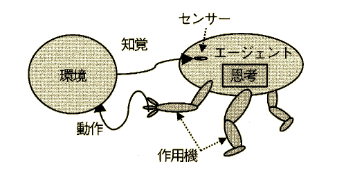
\includegraphics[scale=1.0]{figures/intelligent_agent.png}
 \caption[知的エージェントの模式図]{知的エージェントの模式図 \label{intelligent_agent}}
\end{center}
\end{figure}

\begin{figure}[htb]
\begin{center}
 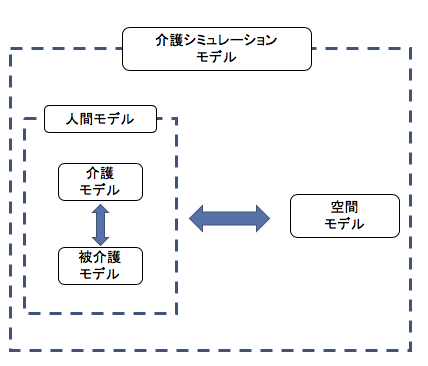
\includegraphics[scale=0.6]{figures/agent_modeling.png}
 \caption[本シミュレーションにおける環境とエージェント]{本シミュレーションにおける環境とエージェント \label{agent_modeling}}
\end{center}
\end{figure}

\subsection{Social force model}

本研究では,高齢者施設内で介護者が高齢者のトイレ介護のために空間移動するプロセスをモデリングするために,Social force model(SFM)\cite{SFM}という歩行者モデリング理論を用いる.Social Force Modelは,歩行者を2次元の粒子であると仮定し,その粒子に以下の4つの力が働くと仮定するモデルである.

\begin{itemize}
 \item 移動目標に近づく力
 \item 他のエージェントからの斥力
 \item 壁などの環境からの斥力
 \item 魅力的な環境への引力
\end{itemize}

移動目標に近づく引力は,エージェントが当初想定していたコースからはずれてしまった場合に目的地の進行方向へと曲げるように働く力のことであり,他のエージェントや壁などからの斥力は,エージェント間,あるいは壁とエージェント間との距離や,お互いの進行方向から決定される反発的な力のことである.魅力的な環境への引力では,友人やショーウィンドー,高齢者支援施設の中では手すりのような,歩行者にとって近づくことのインセンティブが発生するようなものへの引力のことである.これら4つの力は以下のように数式で表現される.

\begin{equation}
\begin{split}
 F_α(t)=F_α^o(υ_α,υ_α^0e_α)&+\sum_{β}F_αβ(e_α,r_α-r_β)\\
 &+\sum_{B}F_αβ(e_α,r_α-r_B^α)\\
 &+\sum_{i}F_αi(e_α,r_α-r_i,t)
\end{split}
\end{equation}

右辺第一項が移動目標に近づく力,第二項が他のエージェントからの斥力,第三項が壁などの環境からの斥力,第四項が魅力的な環境への引力を表している.各エージェントはタイムステップごとに以上の力を計算して,あらかじめ設定された最大歩行速度を超えないように歩行速度を更新する.

\subsection{シミュレーションフロー}

本研究におけるシミュレーションの流れの概略図を図\ref{simulation_flow}に示す。まず、高齢者施設、介護者、被介護者といった空間を構成する要素を環境として構成し、その後実際にシミュレーションを開始する。タイムステップごとに、各エージェントの内部状態を変化させ、介護シミュレーションを行っていく。被介護者の場合は、時間経過で尿量を加算し、エージェントごとに設定されている閾値を超えた時点で介護アラートを出す。介護者は、自分の周りで介護アラートが出たタイミングで、自らと最も距離の近い被介護者のもとへの介護に向かう。これを繰り返すことがシミュレーションが進んで行く。

\begin{figure}[htb]
\begin{center}
 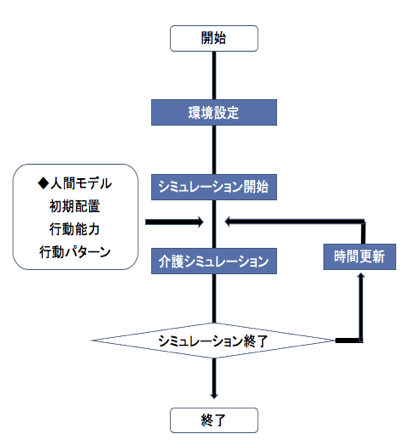
\includegraphics[scale=0.8]{figures/simulation_flow.png}
 \caption[シミュレーションフロー]{シミュレーションフロー \label{simulation_flow}}
\end{center}
\end{figure}

\subsection{介護ペア選択アルゴリズム}

上述のように、被介護者がアラートを発した時にどの介護士とマッチングさせるのかというのがシミュレーション上必要になる。本研究では、各タイムステップごとにある被介護者がアラートを出した時点で、その被介護者と介護可能な介護士との距離を計算し、ペアになりうる介護士と被介護者のペア候補配列を作成していき、その中で全探索を行うことで、最も距離の近いペアを作成して行くこととする。

\section{仮想環境}
本シミュレータにおける環境とは,高齢者施設とそこに存在する介護者、被介護者構造を指す.高齢者施設のモデル化はそれ自体が交通流シミュレータの汎用性・拡張性を実現する上で重要な課題である.本シミュレータでは,介護者・被介護者は基本的に.自由移動を行うことができる二次元平面を想定している。

\subsection{高齢者施設}

今回の開発では,高齢者施設を表現するための第1ステップとして,Social Force Modelを利用するため自由に歩行できる連続空間を対象とし、壁に囲まれた移動可能な二次元平面を作成した。

\subsection{介護者エージェント}

介護者工一ジェントは2次元の高齢者施設に存存するため,方向と速度の制御を行わなければならない.今回は,歩行者の行動モデルとしてSocial Force Modelを採用した.歩行者シミュレーションの研究分野においては、様々なモデル化が検剤されている\cite{ex_pedestrian_simulation_1,ex_pedestrian_simulation_2}.たとえば,磁気モデルを用いると多方向に歩行するエージェントの相互作用を効率的に記述することが可能である.しかし,今回の研究のように閉二次元平面での歩行を対象とする場合には,部屋の中を目的地に対してどう動いて行くかを単純に記述するモデルで十分である.また歩行者モデルとしてあまり複雑なモデルを採用すると計算量が増大しシミュレータの大規模化が困難であることから,本研究ではSocial Force Modelを採用した.以下で歩行者工一ジェントの特徴と挙動について述べる.

\subsection{被介護者エージェント}

被介護者エージェントについては、介護者エージェントと同様にSocial Force Modelを軸に、歩行者エージェントを作成し、それに加えてエージェントの状態によって時系列的に発生する要介護行動を実装した.高齢者の排尿に関する実態研究 \cite{micturition} によると、排尿障害症状を自覚している人は男子が38%、女子が23%と高い水準にあり、男子では排尿困難症状が多く、女子では頻尿を訴える例が多かった。また明らかな尿失禁を抱えているのにも関わらず、その存在を知られたくないという心理が半数以上の人に認められたことも挙げられている。これらから、実際にトイレに行きたいと思っているかどうかの認知についてと、トイレで正常に排尿を行えるのかどうかといった機能について、被介護者のバリエーションを設けることとした.
